\section{Product installation and setup}
  \subsection{Requirements}
    This section describes all of the basic requirements needed to run and test the product.
    \subsubsection{Hardware requirements}
      \begin{itemize}
      	\item \textbf{Internet connection}: needed for the interaction with the Ethereum$_{G}$ blockchain$_{G}$ and AWS.
      \end{itemize}
    \subsubsection{Software requirements}
      \begin{itemize}
        \item \textbf{Node.js$_{G}$:} version 12.0.0 or higher is required. Download and install the latest version from the \href{https://nodejs.org/it/download/}{Node official site};
        \item \textbf{npm (Node Package Manager):} version 6.10.0 or higher is required. It comes with the installation of Node.
        \item \textbf{Git$_{G}$:} a working version of git that can be found at \href{https://git-scm.com/book/en/v2/Getting-Started-Installing-Git}{How to install Git}.
      \end{itemize}
    \subsubsection{General requirements}
      In order to interact with the Ethereum$_{G}$ network an Ethereum$_{G}$ account is needed. The account needs to have a positive balance so that functionality costs can be covered. With \textit{Etherless} a wallet on the run can be created, but it does not contain any Ethers$_{G}$.
  \subsection{Installation}
    The following instructions are to be intended for use on a Unix-based system. Instructions for use on different systems will be added in the future.
    \subsubsection{Download the application}
      A copy of Etherless-cli can be downloaded from the corresponding GitHub repository. Follow the steps below to set up the application:
      \begin{itemize}
        \item download a zip of the repository from \href{https://github.com/RoundaboutTeam/etherless-cli/tree/master}{Etherless-cli}, as shown in the image below;
        \begin{figure}[H]
    			\centering
    			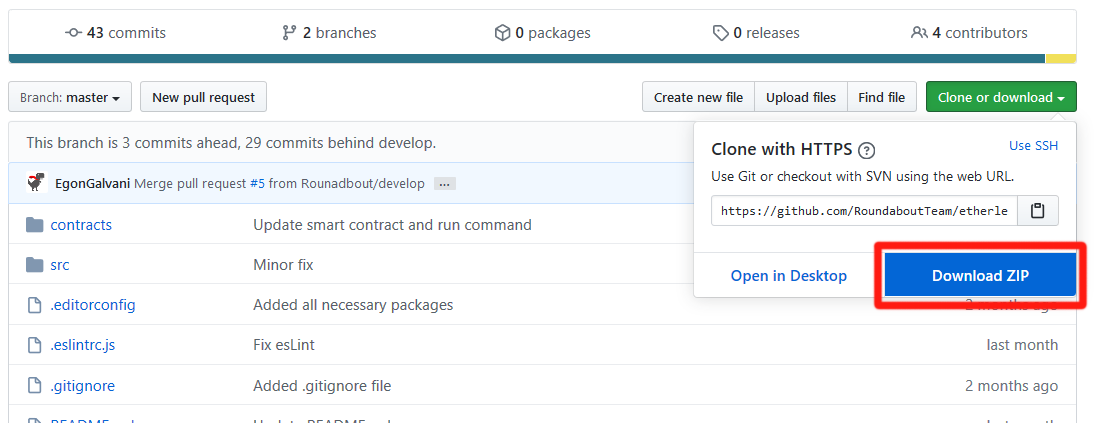
\includegraphics[width=1.1\textwidth]{./res/img/down_zip_repo.png}
    			\caption{Download zip button}
    		\end{figure}
        \item unzip the files in a directory of your choice;
        \item open a terminal as administrator and move to the chosen directory, where you unzipped the files;
        \item run the command \texttt{npm install} to install the dependencies;
        \item run the command \texttt{npm link} to make the \texttt{etherless} commands available.
      \end{itemize}
      \textbf{Note:} we are working towards a more streamlined installation process.
    \subsubsection{Usage}
      The next section describes all the application's functionalities and how to run them. You will make use of the specific commands described to make use of its features.
